%%%%%%%%%%%%%%%%%%%%%%%%%
\section{Experiments and Results}

\subsection{Experimental Setup}

\noindent\textbf{Datasets.} We consider the problem of finding social influencers in two domains: fashion and information technology (InfoTech). For both domains, we publish question-answering tasks in Figure Eight\footnote{\url{https://www.figure-eight.com}} and collect crowd workers' answers. Key statistics of these datasets are reported in Table~\ref{tab:datasets}. For both datasets, we randomly select 40\% of the candidate influencers and ask domain experts to label them. Our initial analysis reveals that 30.64\% and 32.78\%  of the crowd answers are true influencers for Fashion and InfoTech, respectively. Considering the relatively large number of crowd answers collected in a short period of time ($<$10 hours for both Fashion and InfoTech), this result validates our assumption that crowdsourced open-ended question-answering provides an efficient way for finding social influncers. Moreover, the high sparsity of the answer matrices (Table~\ref{tab:datasets}) and the fact that the majority of the answers being incorrect verify the necessity of open-ended answers aggregation that takes into account worker reliability.

\begin{table}[!ht]
%\small
\centering \caption{Descriptive statistics of the
datasets.}\label{tab:datasets}
%\vspace{-0.05in}
\addtolength{\tabcolsep}{-1mm}
\begin{tabular}{lcccc}
\toprule
    Datasets & \textbf{\#Cand. Infl.} & \textbf{\#Workers} & \textbf{\#Answers} & \textbf{Sparsity}   \\\midrule
    Fashion & 890 & 250 & 1416  & 99.36\% \\
    InfoTech & 1057 & 200 &1643 & 99.22\% \\
\bottomrule
\end{tabular}
% \vspace{-0.1in}
\end{table}

\begin{table*}[t]
\centering
\caption{Performance (accuracy and AUC) comparison of aggregation techniques on two datasets with supervision degree $s\_deg$ from 50\% to 90\%. The best performance is highlighted in bold; and the second best performance is marked by `*' for accuracy and by `+' for AUC.}\label{tab:comparision} 
\begin{tabular}{ll|ccccc|ccccc}
\toprule
\multirow{2}{*}{\textbf{Method}}  &   \multirow{2}{*}{\textbf{Metric}}  & \multicolumn{5}{|c|}{\textbf{Fashion}}      & \multicolumn{5}{c}{\textbf{InfoTech}}  \\ \cline{3-12}
 & &   50\%           & 60\%           & 70\%           & 80\%           & 90\%           & 50\%           & 60\%           & 70\%           & 80\%           & 90\%           \\ \midrule
\multirow{2}{*}{DS}          & Accuracy     & 0.689          & 0.716*         & 0.703          & 0.688          & 0.711         & 0.662          & 0.660          & 0.626          & 0.641          & 0.536          \\ % \cline{2-12} 
                             & AUC   & 0.191          & 0.169          & 0.242+          & 0.244          & 0.263          & 0.174          & 0.203+         & 0.222+         & 0.255          & 0.272          \\ \hline
\multirow{2}{*}{GLAD}        & Accuracy     & 0.697          & 0.716*         & 0.724          & 0.700          & 0.688          & \textbf{0.669}        & 0.667          & 0.637          & 0.672          & 0.595          \\ %\cline{2-12} 
                             & AUC   & 0.183          & 0.189          & 0.229          & 0.224          & 0.263          & 0.150          & 0.186          & 0.138          & 0.219          & \textbf{0.307}         \\ \hline
\multirow{2}{*}{ZenCrowd}                           & Accuracy     & 0.701          & 0.686          & 0.733* & 0.702*         & 0.688          & 0.651          & 0.674*         & 0.664* & 0.683* & 0.627*         \\ %\cline{2-12} 
                             & AUC   & 0.157          & 0.175          & 0.203         & 0.239          & 0.287+         & 0.146          & 0.198          & 0.212          & 0.246          & 0.234          \\ \hline
\multirow{2}{*}{LFC}         & Accuracy     & 0.721*         & 0.694          & 0.718          & 0.691          & 0.755*          & 0.653          & 0.627          & 0.643          & 0.616          & 0.636          \\ %\cline{2-12} 
                             & AUC   & 0.203+         & 0.203+         & 0.225          & 0.264+         & 0.277          & 0.189+         & 0.192          & 0.215          & 0.276+         & \textbf{0.307}         \\ \hline
\multirow{2}{*}{OpenCrowd}   & Accuracy     & \textbf{0.733} & \textbf{0.740} & \textbf{0.751}         & \textbf{0.769} & \textbf{0.889}  & 0.666* & \textbf{0.676} &\textbf{0.687}         & \textbf{0.697}         & \textbf{0.742} \\ % \cline{2-12} 
                             & AUC   & \textbf{0.304} & \textbf{0.350} & \textbf{0.350} & \textbf{0.452} & \textbf{0.495} & \textbf{0.268} & \textbf{0.259} & \textbf{0.280} & \textbf{0.280}  &  0.301*\\ \bottomrule
\end{tabular}
 \label{sec:compres}  
\end{table*}

\smallskip
\noindent\textbf{Comparison Methods.} Due to the lack of existing open-ended answers aggregation methods, we compare with the following state-of-the-art closed-pool answers aggregation methods: 1) ZenCrowd \cite{demartini2012zencrowd}, an EM method that estimates worker reliability as a model parameter; 2) Dawid-Skene \cite{dawid1979maximum}, an EM method that learns worker reliability as a confusion matrix; 3) GLAD \cite{whitehill2009whose}, an EM method that simultaneously learns worker reliability and task difficulty; and 4) LFC \cite{raykar2010learning}, an EM method 
that incorporates priors in modeling worker reliability. To apply these methods to our problem, we use negative sampling to simulate workers' answers of non-influencers; we empirically determine the optimal sampling rates for each comparison method. 

To investigate the benefit of modeling worker reliability as compared to feature-based methods, we compare our technique against logistic regression (LR) and multi-layer perceptron (MLP). We define two variants of our framework: 1) \sys-EM: \sys that aggregates workers' answers however models worker reliability as a fixed paramter; and 2) \sys, the Bayesian version that models worker reliability as a latent variable.




\smallskip
\noindent\textbf{Parameter Settings.} The parameters of our framework and those for model training are empirically set. We search for the best model architecture for MLP, and the predictor $f$ in \sys-EM and \sys, with 0, 1, and 2 hidden layers, and apply a grid search in \{64, 128, 256, 512, 1024\} for the dimension of the hidden layers. In model training, we select learning rates from \{0.0001, 0.001, 0.01, 0.1, 1\} for the learning of $\mathbf{W}_I$ in all variants of our framework, as well as for the learning of $r_j$ in \sys-EM. To investigate the impact of negative sampling, we experiment with sampling rate ($s\_rate$) from \{0, 0.1, 1, 10, 100\} where $s\_rate=10$ indicates that for each worker, the negative samples is ten times the size of the candidate influencers named by each worker. 

\smallskip
\noindent\textbf{Evaluation Protocols.} We split the labeled subset of candidate influencers into training, validation, and test sets. \sys is trained on the answers and the training set, tuned on the valiation set and evaluated on the test set. To investigate the impact of the degree of supervision ($s\_deg$) on \sys performance, we split the labeled subset by $s\_deg\in \{50\%, 60\%, 70\%, 80\%, 90\%\}$, where $s\_deg = 60\%$ means that 60\% of the labeled subset is used for training, and the rest for validation and test with equal split. We use accuracy and area under the precision-recall curve (AUC) to measure the performance. Higher values of accuracy and AUC indicate better performance.



\subsection{Comparative Results}
Table~\ref{sec:compres} summarizes the performance of the compared answers aggregation methods on the two datasets with different supervision degree. Several interesting findings are observed.

First, we observe that ZenCrowd generally outperforms DS and GLAD. Recall that ZenCrowd is less expressive compared to DS and GLAD, as it only models worker reliability as a parameter. In comparison, DS models worker reliability as a confusion matrix, and GLAD further models the task difficulty (in our context the ambiguity of a candidate influencer being the true influencer). The superior performance of ZenCrowd  over DS and GLAD indicates that in our context, more expressive models do not necessary lead to higher performance. This is likely due to the high sparsity of worker-answer matrices (Table~\ref{tab:datasets}) that can easily lead to overfitting.

Second, we observe that methods that model worker reliability as a latent variable with a prior distribution, namely LFC and our framework \sys, outperform the other methods. Such a result confirms the necessity of modeling worker reliability as a latent variable, as it helps to account for the confidence of estimating model parameters. This is particularly important to improve model robustness for sparse datasets as in our case. We  will give more results on this point in Section~\ref{sec:selfres}.

Most importantly, our framework \sys achieves the best performance among all answers aggregation methods under comparison: \sys improves the state of the art by 6.94\% accuracy and 61.99\% AUC on Fashion, and by 4.40\% accuracy and 18.97\% AUC on InfoTech. The big improvements clearly demonstrate the effectiveness of our framework in open-ended answers aggregation. 



\smallskip
\noindent\textbf{Impacts of Supervision Degree.} The supervision degree $s\_deg$ controls the amount of observed labels in model training. We observe that the performance of our framework increases along with the increase of $s\_deg$, as measured by both accuracy and AUC. This is natural as more labeled data provides more information in discriminating influencers from non influencers. Such a pattern, however, is not observed for the other methods that we compare to. This is likely due to the fact that the other methods do not take advantage of the social features, which are useful as they serve as means to propagate the labels to non-labeled candidate influencers. These results, therefore, show that \sys is better at utilizing existing labels for answers aggregation. 

\subsection{Results of \sys}
\label{sec:selfres}

\noindent\textbf{Results of \sys Variants.}
The comparison between \sys variants against feature-based methods is shown in Figure \ref{fig:variants}. \sys-EM outperforms both LR and MLP by 13.05\% and 19.95\% accuracy and by 23.23\% and 25.46\% AUC, respectively. These results clearly show the importance of considering worker reliability in aggregating workers' answers. Among the two variants, \sys outperforms \sys-EM by 1.7\% accuracy and XX\% AUC. This result indicates that modeling the worker reliability as a latent variable with a prior distribution not only makes the model more robust, but also improves the aggregation performance in terms of accuracy and AUC. 

\begin{figure}[htb]
\begin{subfigure}[t]{0.33\columnwidth}
        \centering
    \pgfplotstableread[row sep=\\,col sep=&]{
       cases & LR & MLP & EM & VEM \\
       Fashion     &0.604166667  & 0.7006  & 0.7333 &0.7555  \\
       InfoTech    & 0.511 & 0.6  & 0.66235&0.6764 \\
    }\mydata

    \begin{tikzpicture}[scale=0.5]
    \begin{axis}[
    ybar,
    bar width=.4cm,
    width=2\textwidth,
    height=1.5\textwidth,
    legend style={at={(1.2,1.35)},
       anchor=north,legend columns= 4, font = \LARGE},
    symbolic x coords={Fashion, InfoTech},
    xtick=data,
    enlarge x limits=0.3,
    ymin=0.4,ymax=0.80,
    ylabel={Accuracy},
    yticklabel style = {xshift=0.5ex},
    xticklabel style = {yshift=0.5ex},
    ylabel style ={yshift=-2ex},
    ymajorgrids=true
    ]
    \addplot[draw=gray,fill=gray!40!white, thick] table[x=cases,y=LR]{\mydata};
    \addplot[draw=blue,fill=blue!40!white] table[x=cases,y=MLP]{\mydata};
    \addplot[draw=black,fill=black!50!white, thick] table[x=cases,y=EM]{\mydata};
    \addplot[draw=red,fill=red!40!white, thick] table[x=cases,y=VEM]{\mydata};
    \legend{LR, MLP, \sys-EM, \sys}
    \end{axis}
    \end{tikzpicture}
    \vspace{-0.15in}
       \caption{Accuracy\label{fig:acc}} 
    \end{subfigure}% 
  \hfill \hskip -4ex %
    	\begin{subfigure}[t]{0.33\columnwidth}
        \centering
  \centering
    \pgfplotstableread[row sep=\\,col sep=&]{
       cases & LR & MLP & EM & VEM \\
       Fashion     &0.235142445  & 0.2154  &0.277139619 &0.42670444  \\
       InfoTech   &0.18673464  & 0.2154  & 0.251&0.259 \\
    }\mydata

    \begin{tikzpicture}[scale=0.5]
    \begin{axis}[
    ybar,
    bar width=.4cm,
    width=2\textwidth,
    height=1.5\textwidth,
    legend style={at={(1,1.5)},
       anchor=north,legend columns= 4, font = \LARGE},
    symbolic x coords={Fashion, InfoTech},
    xtick=data,
    enlarge x limits=0.3,
    ymin=0.1,ymax=0.5,
    ylabel={AUC},
    yticklabel style = {xshift=0.5ex},
    xticklabel style = {yshift=0.5ex},
    ylabel style ={yshift=-2ex},
    ymajorgrids=true
    ]
    \addplot[draw=gray,fill=gray!40!white, thick] table[x=cases,y=LR]{\mydata};
    \addplot[draw=blue,fill=blue!40!white] table[x=cases,y=MLP]{\mydata};
    \addplot[draw=black,fill=black!50!white, thick] table[x=cases,y=EM]{\mydata};
    \addplot[draw=red,fill=red!40!white, thick] table[x=cases,y=VEM]{\mydata};
    \legend{}
    \end{axis}
    \end{tikzpicture}
        \caption{AUC\label{fig:AUC}} 
    \end{subfigure}% 
     \hfill \hskip -4ex %
    	\begin{subfigure}[t]{0.33\columnwidth}
        \centering
        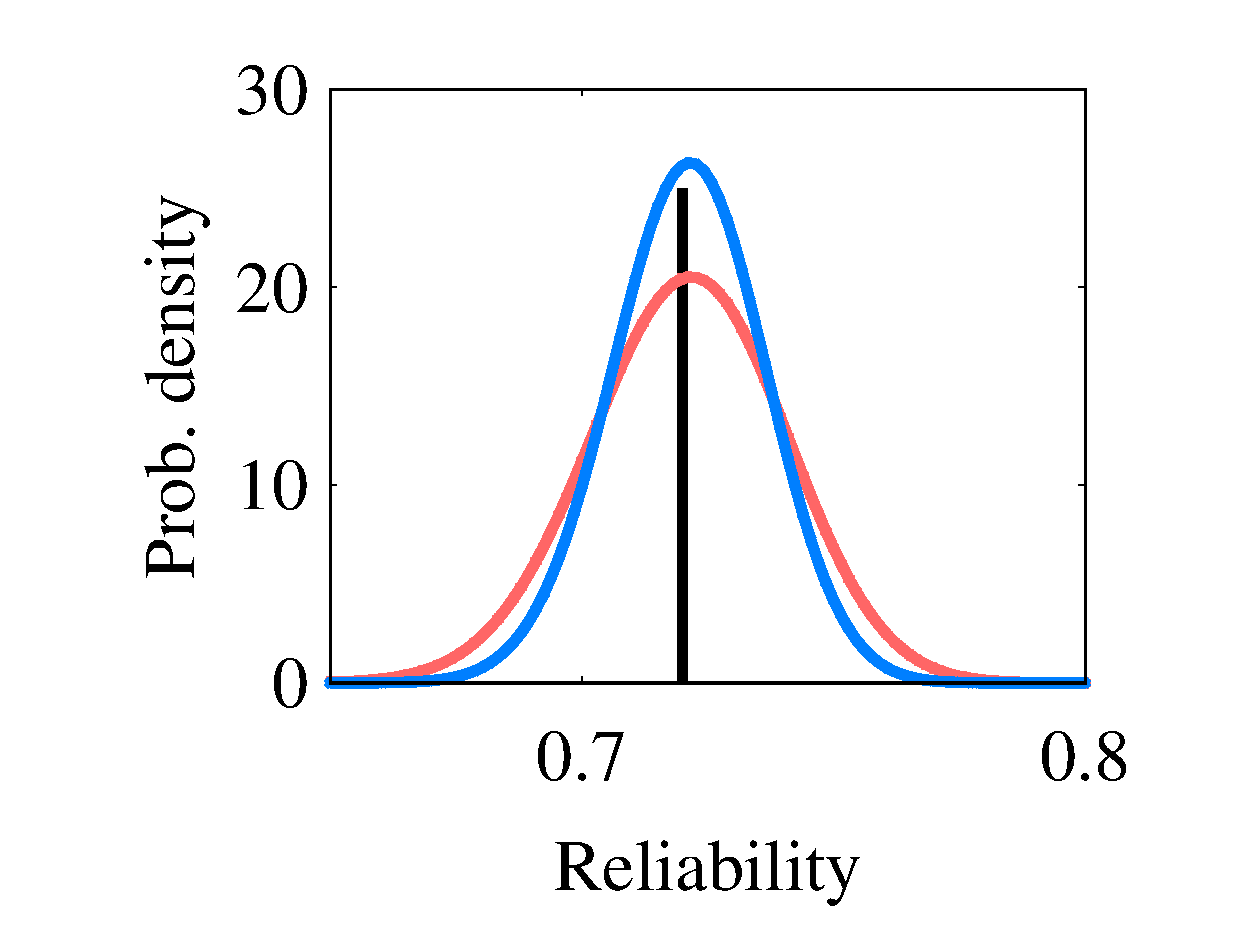
\includegraphics[width=\columnwidth]{figs/beta_dist.eps}
        \caption{Reliability dist.}\label{fig:worker_reliability}
    \end{subfigure}
   \caption{Performance of our four variants.} \label{fig:variants} 
\end{figure}

To quantitatively show the effect of modeling worker reliability as a latent variable, we depict in Figure~\ref{fig:worker_reliability} two examples of workers of similar reliability yet providing different number of answers. We observe that their reliability, as estimated by \sys-EM, are hardly distinguiable; however, \sys provides extra insight that the estimated reliability of the left worker is more trustable than that of the right worker.




\smallskip
\noindent\textbf{Impacts of Sampling Rate.}
The sampling rate $s\_rate$ controls the size of randomly sampled candidate influencers in estimating workers' reliability. The results are shown in Figure~\ref{fig:sys_perf_it}. We observe that, as the sampling rate varies from 0 to 100, the performance first increases then decreases. Such a result is consistent on both datasets, measured by both accuracy and AUC. The maximum performance is reached for $s\_rate= 10$ for Fashion and $s\_rate= 0.1$ for InfoTech, indicating that workers' evaluation about the candidate influencers they do not name is more negative in Fashion. Overall, the variation of the performance with different $s\_rate$ indicates the importance of selecting the optimal sampling rate. The similarity in performance variation across the two datasets demonstrates the robustness of \sys.

\begin{figure}[htb]\centering
	\begin{subfigure}[t]{0.47\columnwidth}
\begin{tikzpicture}[scale=0.5]
\begin{axis}[
    xlabel={Sampling Rate},
    ylabel={Accuracy},
    xmin=0, xmax=100,
    ymin=0.55, ymax=0.8,
    xtick={0,25,50,75,100},
    xticklabels={$0$,$0.1$,$1$,$10$,$100$},
    ytick={0.6,0.65,0.7,0.75,0.8},
       legend style={at={(1.15,1.2)},
       anchor=north,legend columns= 4, font = \LARGE},
    yticklabel style = {font=\huge,xshift=0.5ex},
    xticklabel style = {font=\huge,yshift=0.5ex},
    ylabel style ={font = \huge},
    xlabel style ={font = \huge},
    ymajorgrids=true,
    grid style=dashed,
    width=2\textwidth,
    height=1.5\textwidth
]
\addplot[
    color=blue,
    mark=square,
    ]
    coordinates 
 {
    (0,0.5861)
    (25,0.615)
    (50,0.625)
    (75,0.7027)
    (100,0.6944)
    };
   \addplot plot coordinates {
            (0,   0.625)
            (25,0.6347)
            (50,   0.63611)
            (75, 0.75555)
             (100,  0.6805555)
        };   
\legend{\sys-EM, \sys}
\end{axis}
\end{tikzpicture}
    \vspace{-0.15in}
        \caption{Fashion - Accuracy\label{fig:acc_sr}} 
 \end{subfigure}
 \begin{subfigure}[t]{0.47\columnwidth}
\begin{tikzpicture}[scale=0.5]
\begin{axis}[
    xlabel={Sampling Rate},
    ylabel={AUC},
    xmin=0, xmax=100,
    ymin=0.2, ymax=0.45,
    xtick={0,25,50,75,100},
    xticklabels={$0$,$0.1$,$1$,$10$,$100$},
    ytick={0.2,0.25,0.3,0.35,0.4,0.45},
       legend style={at={(0.67,1.2)},
       anchor=north,legend columns= 4, font = \LARGE},
    yticklabel style = {font=\huge,xshift=0.5ex},
    xticklabel style = {font=\huge,yshift=0.5ex},
    ylabel style ={font = \huge},
    xlabel style ={font = \huge},
    ymajorgrids=true,
    grid style=dashed,
    width=2\textwidth,
    height=1.5\textwidth
]
\addplot[
    color=blue,
    mark=square,
    ]
    coordinates 
 {
(0,	0.2125)
(25, 0.2293)
(50,	0.23116	)
(75,	0.25349)
(100,	0.3486560	)
    };
   \addplot plot coordinates {
(0	,	0.33)
(25,0.34)
(50,	0.35039)
(75	,	0.35039)
(100	,0.350547	)
        };   
\legend{}
\end{axis}
\end{tikzpicture}
    \vspace{-0.15in}
        \caption{Fashion - AUC\label{fig:AUC_sr}} 
 \end{subfigure}
   
	\begin{subfigure}[t]{0.47\columnwidth}
\begin{tikzpicture}[scale=0.5]
\begin{axis}[
    xlabel={Sampling Rate},
    ylabel={Accuracy},
    xmin=0, xmax=100,
    ymin=0.55, ymax=0.8,
    xtick={0,25,50,75,100},
    xticklabels={$0$,$0.1$,$1$,$10$,$100$},
    ytick={0.55,0.6,0.65,0.7,0.75,0.8},
       legend style={at={(0.67,1.2)},
       anchor=north,legend columns= 4, font = \LARGE},
    yticklabel style = {font=\huge,xshift=0.5ex},
    xticklabel style = {font=\huge,yshift=0.5ex},
    ylabel style ={font = \huge},
    xlabel style ={font = \huge},
    ymajorgrids=true,
    grid style=dashed,
    width=2\textwidth,
    height=1.5\textwidth
]
\addplot[
    color=blue,
    mark=square,
    ]
    coordinates 
 {
(0,	0.673	)
(25,	0.681)	
(50, 0.682)
(75, 0.560)	
(100,0.574)	
    };
   \addplot plot coordinates {
(0	,	0.765)
(25	,	0.7777)
(50	,	0.727)
(75	,	0.6015)
(100,	0.6078)
        };   
\legend{}
\end{axis}
\end{tikzpicture}
    \vspace{-0.15in}
        \caption{InfoTech - Accuracy\label{fig:acc_sr_it}} 
 \end{subfigure}
 \begin{subfigure}[t]{0.47\columnwidth}
\begin{tikzpicture}[scale=0.5]
\begin{axis}[
    xlabel={Sampling Rate},
    ylabel={AUC},
    xmin=0, xmax=100,
    ymin=0.1, ymax=0.4,
    xtick={0,25,50,75,100},
    xticklabels={$0$,$0.1$,$1$,$10$,$100$},
    ytick={0.1,0.15,0.2,0.25,0.3,0.35},
         legend style={at={(0.67,1.2)},
       anchor=north,legend columns= 4, font = \LARGE},
    yticklabel style = {font=\huge,xshift=0.5ex},
    xticklabel style = {font=\huge,yshift=0.5ex},
    ylabel style ={font = \huge},
    xlabel style ={font = \huge},
    ymajorgrids=true,
    grid style=dashed,
    width=2\textwidth,
    height=1.5\textwidth
]
\addplot[
    color=blue,
    mark=square,
    ]
    coordinates 
 {
(0,		0.257)
(25	,	0.2755)
(50,0.302)
(75 , 0.26)
(100,0.253)
    };
   \addplot plot coordinates {
(0,		0.323)
(25	,	0.324)
(50 , 0.313)
(75,0.3037)
(100,0.2166)
        };   
\legend{}
\end{axis}
\end{tikzpicture}
 \caption{InfoTech - AUC\label{fig:AUC_sr_it}} 
 \end{subfigure}
   \caption{Performance of \sys with varying $s\_rate$.}\label{fig:sys_perf_it} 
\end{figure}

